\begin{figure}[H]
	\centering
	\includegraphics[width=\textwidth]{figures/all_maps.png}
	\caption{Maps of the islands. (A) Map of the West Indies with sampled islands highlighted in black. (B) Sampling sites within islands colored after their respective habitat-types.}
	\label{fig:maps}
\end{figure}

\begin{figure}[H]
	\centering
	\includegraphics[width=\textwidth]{figures/Bimini.png}
	\caption{Comparison of dewlap coloration across habitats on Bimini. Legend is as per Figure \ref{fig:Abaco}.}
	\label{fig:Bimini}
\end{figure}

\begin{figure}[H]
	\centering
	\includegraphics[width=\textwidth]{figures/CaymanBrac.png}
	\caption{Comparison of dewlap coloration across habitats on Cayman Brac. Legend is as per Figure \ref{fig:Abaco}.}
	\label{fig:CaymanBrac}
\end{figure}

\begin{figure}[H]
	\centering
	\includegraphics[width=\textwidth]{figures/Eleuthera.png}
	\caption{Comparison of dewlap coloration across habitats on Eleuthera. Legend is as per Figure \ref{fig:Abaco}.}
	\label{fig:Eleuthera}
\end{figure}

\begin{figure}[H]
	\centering
	\includegraphics[width=\textwidth]{figures/LittleCayman.png}
	\caption{Comparison of dewlap coloration across habitats on Little Cayman. Legend is as per Figure \ref{fig:Abaco}.}
	\label{fig:LittleCayman}
\end{figure}

\begin{figure}[H]
	\centering
	\includegraphics[width=\textwidth]{figures/LongIsland.png}
	\caption{Comparison of dewlap coloration across habitats on Long Island. Legend is as per Figure \ref{fig:Abaco}.}
	\label{fig:LongIsland}
\end{figure}

\begin{figure}[H]
	\centering
	\includegraphics[width=\textwidth]{figures/NorthAndros.png}
	\caption{Comparison of dewlap coloration across habitats on North Andros. Legend is as per Figure \ref{fig:Abaco}.}
	\label{fig:NorthAndros}
\end{figure}

\begin{figure}[H]
	\centering
	\includegraphics[width=\textwidth]{figures/SouthAndros.png}
	\caption{Comparison of dewlap coloration across habitats on South Andros. Legend is as per Figure \ref{fig:Abaco}.}
	\label{fig:SouthAndros}
\end{figure}

\begin{figure}[H]
	\centering
	\includegraphics[width=0.8\textwidth]{figures/brightness.png}
	\caption{PC1 captures brightness across all islands. (A) Correlation between dewlap brightness (as measured by the mean reflectance from 300 to 700nm in wavelength) and PC1 score across all islands. (B) Correlation between brightness and within-island PC1, for each island. Pearson's correlation coefficients are reported. ***, $P < 0.001$.}
	\label{fig:brightness}
\end{figure}
